\documentclass[11pt]{article}
\usepackage[utf8]{inputenc}
\usepackage[ngerman]{babel}

\usepackage{amsmath,amsthm,amssymb,amsfonts}

\usepackage{graphicx}
\graphicspath{{abb/}}
\usepackage{float}
\usepackage{tikz}

\usepackage{fancyhdr} % For headers and footers
\usepackage{geometry}
\usepackage{listings}
\usepackage{hyperref}
\hypersetup{
    linkcolor=blue,     
    urlcolor=cyan,
}

\geometry{
    a4paper, % Change this if you intend to print on a different paper size, such as letter paper.
    left=20mm,
    right=20mm,
    top=30mm,
    bottom=30mm,
}

\title{Kinematik in einer Raumrichtung - konstante Geschwindigkeit}
\author{Emil Staikov}
\date{12. Februar 2021}

\begin{document}
\maketitle
\section{Definitionen erster Größen}
In der Kinematik betrachten wir die Bewegungen von Körpern ohne ihre Ursache, heißt wir versuchen Ort, Geschwindigkeit und Beschleunigung eines Körpers aus anderen gegebenen Größen zu finden. Zuerst müssen wir die Größen der Kinematik definieren: \\

Der Ort $s$ beschreibt, wo wir uns im Raum befinden. Im eindimensionalen Fall ist er der Abstand zu einem fest gewählten Punkt, dem Koordinatenursprung. Meist wählen wir den Anfangspunkt unserer Bewegung als Korrdinatenursprung. \\

Die Geschwindigkeit ist die Änderung des Ortes in einem Zeitabschnitt. Wenn wir zum Zeitpunkt $t_1$ am Ort $s_1$ sind und am Zeitpunkt $t_2$ am Ort $s_2$, dann ist unsere Durchschnittsgeschwindigkeit in diesem Zeitabschnitt definiert als
$$ v = \frac{s_2-s_1}{t_2-t_1} = \frac{\Delta s}{\Delta t}$$ 
Je kleiner der Zeitabschnitt $\Delta t$ ist, den wir betrachten, also je näher $t_2$ an $t_1$ ist, desto näher kommen wir der Geschwindigkeit in dem Moment $t_1$ (und dem Ort $x_1$). Für die genaue Definition der Momentangeschwindigkeit brauchen wir die Methoden der Differentialrechnung, bei der IJSO wird diese jedoch nicht benötigt. \\

Die Beschleunigung definieren wir später. \\

\section{Die geradlinig gleichförmige Bewegung}
Wir unterscheiden verschiedene Bewegungsarten, dabei ist die grundlegendste die geradlinig-gleichfömige Bewegung (GGB). Bei dieser bewegen wir uns auf einer geraden Linie mit einer gleichbleibenden Geschwindigkeit, nach der Definition der Geschwindigkeit gilt $$v = \frac{\Delta s}{\Delta t}$$ In diesem Sonderfall der Bewegung ist die Durchschnittsgeschwindigkeit gleich der Momentangeschwindigkeit in jedem Moment, da die Geschwindigkeit stets gleich bleibt. Wir können die Geschwindigkeit ebenfalls als konstante Funktion $v(t)$ in einem Koordinatensystem aufzeichnen: 
\begin{figure}[H] 
  \centering
     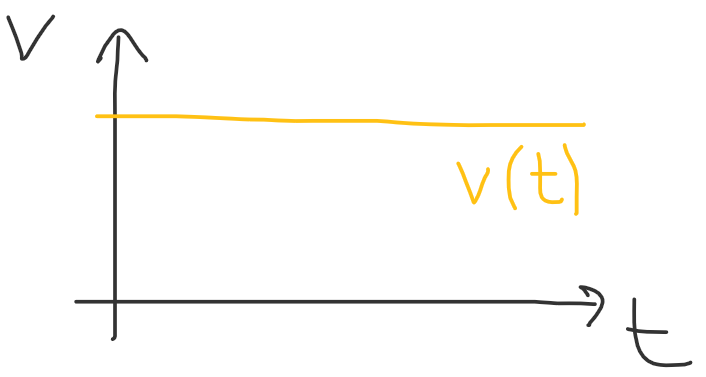
\includegraphics[width=0.6\textwidth]{v-t-diagramm-ggb.png}
     \caption{v-t-Diagramm einer GGB}
\end{figure} 
Nun wollen wir die Funktion des Ortes in Abhängigkeit von der Zeit und der Geschwindigkeit finden: $$v = \frac{\Delta s}{\Delta t} = \frac{s(t) - s_0}{t - t_0} \Longleftrightarrow s(t) = v(t - t_0) + s_0 = v \Delta t + s_0$$
$s(t)$ gibt uns den gereisten Weg, wenn wir am Punkt $s_0$ starten, und uns über eine Zeit $t$ mit der Geschwindigkeit $v$ bewegen. Die Anfangszeit $t_0$ wählt man meist als $0$, der Ort $s_0$ ist unsere Position am Anfang der Bewegung relativ zum Koordinatenursprung (einem fest gewählten Punkt auf der Gerade). Bewegungen sind immer bezüglich eines Punktes (wenn man keinen Bezugspunkt hat, kann man keine Entfernungen, Geschwindigkeiten etc. messen), diesen Punkt können wir jedoch beliebig wählen. Oft bietet es sich an, den Startpunkt unserer Bewegung als den Koordinatenursprung zu wählen, dann gilt $s_0 = 0$. Mit diesen Überlegungen:
$$s(t) = vt+s_0 \text{, für } (t_0, s_0) = (0, 0): s(t) = vt$$
Das ist eine lineare Funktion in $t$ mit Anstieg $\displaystyle v = \frac{\Delta s}{\Delta t}$, grafisch: 
\begin{figure}[H] 
  \centering
     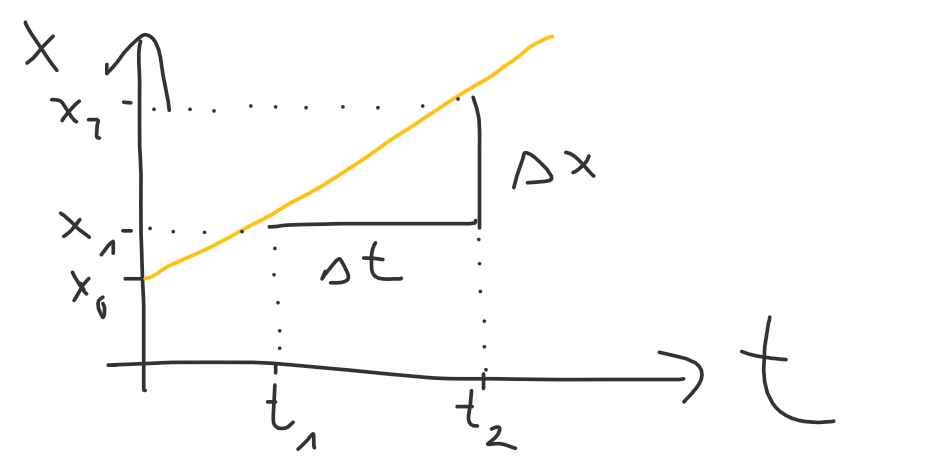
\includegraphics[width=0.6\textwidth]{x-t-diagramm-ggb.png}
     \caption{x-t-Diagramm einer GGB (x entspricht hier s)}
\end{figure} 
Betrachten wir nun die Fläche unter der Geschwindigkeitsfunktion $v(t)$ im v-t-Diagramm der Bewegung während eines Zeitabschnitts $\Delta t$: 
\begin{figure}[H] 
  \centering
     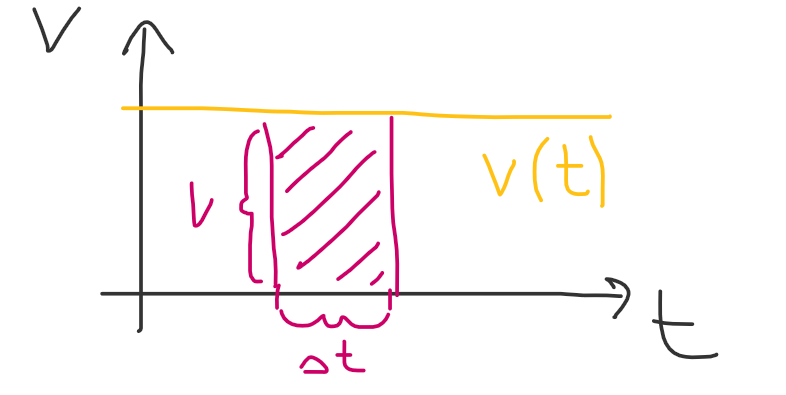
\includegraphics[width=0.6\textwidth]{v-t-diagramm-ggb-mit-flaeche.png}
     \caption{Fläche unter einem v-t-Diagramm}
\end{figure} 
$v(t)$ grenzt stets Rechtecke ein, die Fläche dieser Rechtecke berechnet sich mit $A_{Rechteck} = ab$ zu $A_{v(t)} = v\Delta t$. Das ist jedoch genau der zurückgelegte Weg im Zeitintervall $\Delta t$:
$$\Delta s = s - s_0 = v \Delta t$$
Nochmal in Worten: Die Fläche unter dem Graphen von $v(t)$ ist gleich der in dem Zeitabschnitt zurückgelegten Strecke!

\subsection*{Aufgaben}
Hier einige Aufgaben, um den Umgang mit den Gleichungen zu üben. \\

1.: Überprüft die Einheiten bzw. Dimensionen in allen bisherigen Gleichungen, $[v] = 1 m/s$, $[s] = 1 m$, $[t] = 1s$ ($[x]$ bezeichnet die Einheit der Größe $x$) \\

2.: Betrachten wir wieder einmal unseren Schwimmer: \\
a) Er bewegt sich mit einer Geschwindigkeit $v = 3 m/s$ in einem Becken der Länge $0.05km$. Wie lange braucht er von einem bis zum anderen Beckenrand? \\
b) Wenn er in $0.5h$ von einem bis zum anderen Beckenrand, wie schnell bewegt er sich dann? \\
c) Überlegt euch, wie ihr in a) und b) den Koordinatenursprung gewählt habt. Berechnet a) und b) erneut, aber mit dem Koordinatenursprung in der Mitte des Beckens. Überlegt euch dazu zuerst, wie groß $s_0$ ist, achtet auf die Vorzeichen. Vergleicht die Größen mit den in a) und b) berechneten Werten. \\

3.: Ein Zug startet in A mit Geschwindigkeit $v_A$, ein anderer in B mit Geschwindigkeit $v_B$. Der Abstand zwischen A und B ist $s_{AB}$. Überlege dir, was verschiedene Vorzeichen bei den jeweiligen Geschwindigkeiten bedeuten. \\ 
a) Sie treffen sich nach einer Zeit $t$, leite einen Ausdruck für den Abstand zwischen A und B her. \\
b) Sie treffen sich im Abstand $s$ von A. Leite einen Ausdruck für die Zeit bis zum Auftreffen her. \\
c) Gegeben ist jetzt nur die Geschwindigkeit $v_A$, $s_{AB}$ und der Abstand bis zum Auftreffen $s$. Leite einen Ausdruck für $v_B$ her. \\

Die Aufgaben können wir bei Fragen/Interesse in der AG besprechen. 


\end{document}